%%%%%%%%%%%%%%%%%%%%%%%%%%%%%%%%%%%%%%%%%
% a0poster Portrait Poster
% LaTeX Template
% Version 1.0 (22/06/13)
%
% The a0poster class was created by:
% Gerlinde Kettl and Matthias Weiser (tex@kettl.de)
% 
% This template has been downloaded from:
% http://www.LaTeXTemplates.com
%
% License:
% CC BY-NC-SA 3.0 (http://creativecommons.org/licenses/by-nc-sa/3.0/)
%
%%%%%%%%%%%%%%%%%%%%%%%%%%%%%%%%%%%%%%%%%

%----------------------------------------------------------------------------------------
%	PACKAGES AND OTHER DOCUMENT CONFIGURATIONS
%----------------------------------------------------------------------------------------

\documentclass[a0,portrait]{poster}

\usepackage{multicol} % This is so we can have multiple columns of text side-by-side
\columnsep=100pt % This is the amount of white space between the columns in the poster
\columnseprule=3pt % This is the thickness of the black line between the columns in the poster

\usepackage[svgnames]{xcolor} % Specify colors by their 'svgnames', for a full list of all colors available see here: http://www.latextemplates.com/svgnames-colors

\usepackage{times} % Use the times font
%\usepackage{palatino} % Uncomment to use the Palatino font

\usepackage{graphicx} % Required for including images
\usepackage{booktabs} % Top and bottom rules for table
\usepackage[font=small,labelfont=bf]{caption} % Required for specifying captions to tables and figures
\usepackage{amsfonts, amsmath, amsthm, amssymb} % For math fonts, symbols and environments
\usepackage{wrapfig} % Allows wrapping text around tables and figures

\begin{document}

%----------------------------------------------------------------------------------------
%	POSTER HEADER 
%----------------------------------------------------------------------------------------

% The header is divided into two boxes:
% The first is 75% wide and houses the title, subtitle, names, university/organization and contact information
% The second is 25% wide and houses a logo for your university/organization or a photo of you
% The widths of these boxes can be easily edited to accommodate your content as you see fit

\begin{minipage}[b]{0.6\linewidth}
\veryHuge \color{NavyBlue} \textbf{NDNCERT in Identity Manager} \color{Black}\\ % Title
\Huge\textit{A trial to implement an identity manage using NDNCERT in Named Data Networking(NDN)}\\[2cm] % Subtitle
\Large \textbf{Yuyang(Peter) Rong, \\ Arthi Padmanabhan, Zhiyi Zhang, Lixia Zhang}\\[0.5cm] % Author(s)
\Large ShanghaiTech / UCLA \\ [0.4cm] % University/organization
\Large \texttt{PeterRong96@gmail.com} --- +1 (310) 307 9952\\
\end{minipage}
%
\begin{minipage}[b]{0.4\linewidth}
	
\includegraphics[width=\linewidth]{figures/logo.png}\\
\end{minipage}

\vspace{0.7cm} % A bit of extra whitespace between the header and poster content

%----------------------------------------------------------------------------------------

\begin{multicols}{2} % This is how many columns your poster will be broken into, a portrait poster is generally split into 2 columns

%----------------------------------------------------------------------------------------
%	ABSTRACT
%----------------------------------------------------------------------------------------

\color{Navy} % Navy color for the abstract

\begin{abstract}

Security and privacy in networking are gaining more and more attention nowadays. NDN is a newly proposed architecture that has shown great potential in security. In NDN, each packet has to be signed and thus is secured. In this work, we use NDNCERT, a certificate manager, to request and manage certificates that can be used to sign data packets. We would install this manager in cell phones and thus allow other applications like NDNFit to gain certificate through this manager. 

\end{abstract}

%----------------------------------------------------------------------------------------
%	INTRODUCTION
%----------------------------------------------------------------------------------------

\color{SaddleBrown} % SaddleBrown color for the introduction

\section*{Introduction}
NDN requires each data packet to be signed and thus can be verified. However, our ability to verify the data does not necessarily mean that we can trust the signing entity. NDNCERT is a protocol that allows client to request a certificate from Certificate Authority(CA) that can be used to sign packets. Applications like NDNFit can use such a manager to manage other applications. We used NDNFit as a proof-of-concept example to show that NDNCERT can be used in identity manager to help manage and distribute identities.

%----------------------------------------------------------------------------------------
%	OBJECTIVES
%----------------------------------------------------------------------------------------

\color{DarkSlateGray} % DarkSlateGray color for the rest of the content

\section*{Main Objectives}

\begin{enumerate}
\item Use NDNCERT to write identity manager;
\item Explore NDN development on Android and provide experience for other apps;
\item Provide an identity manager to update NDNFit.
\end{enumerate}

%----------------------------------------------------------------------------------------
%	MATERIALS AND METHODS
%----------------------------------------------------------------------------------------

\section*{Packages}

%------------------------------------------------

\subsection*{NDN\cite{zhang2014named}}
\par
	Unlike tradition TCP/IP architecture, in NDN every data is named under a namespace. 
	To request for a piece of data, one can express an interest with data's name inside and wait.
	When an interest is received, the corresponding data should be sent if it exists. 
	The details about the format of the packets can be found in the figure below.
	In this consumer-producer model, each and every data packet has to be signed and thus consumer can verify the integrity of the data.

%------------------------------------------------
\subsection*{NDN Certificate management protocol(NDNCERT)\cite{zhang2017ndncert}}
\par
	NDNCERT is a set of protocols that allows auto certificate management.
	In NDN, everyone has corresponding namespace and the certificate to sign any data produced in this namespace.
	However, this only guarantees the integrity of the data, consumers can not distinguish if the producer of the data is malicious.
	A mechanism is provided in NDNCERT to get certificate from Certificate Authority(CA).
	Making it possible for one entity to trust the other if the data received is signed by a certificate presented by a trustworthy CA.
\par
\begin{minipage}[b]{0.55\linewidth}
	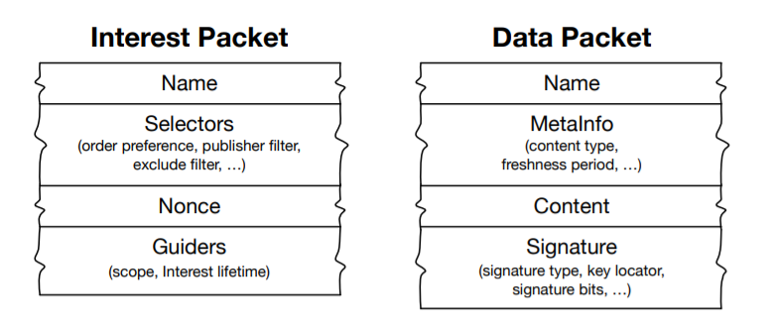
\includegraphics[width=\linewidth]{figures/packet.png}
	\captionof{figure}{packet format in NDN}
	\includegraphics[width=\linewidth]{figures/NDNfit.png}
	\captionof{figure}{NDNFit work flow}
\end{minipage}
\begin{minipage}[b]{0.45\linewidth}
	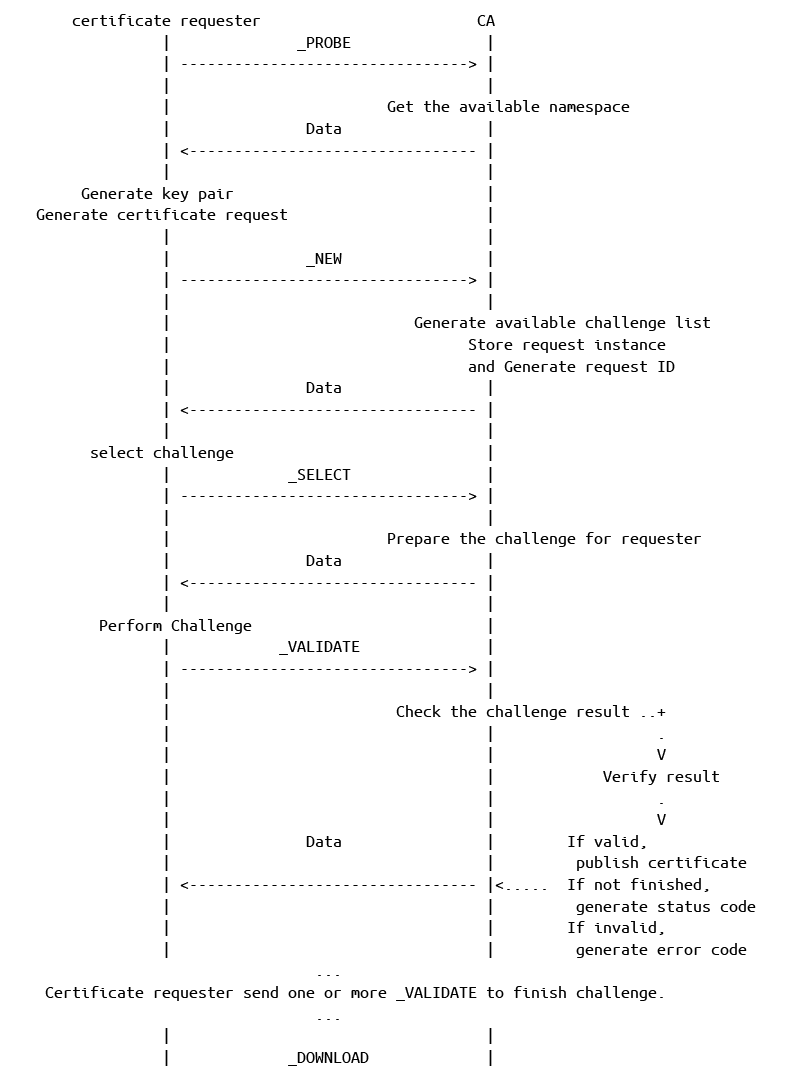
\includegraphics[width=\linewidth]{figures/protocol.png}
	\captionof{figure}{NDNCERT protocol}
\end{minipage}
\par
	In our project, we will be mainly focus on NDNCERT's client part. 
	As we would use NDNCERT client to get a certificate from CA and then manages these identities.
\par
	For each client to get a certificate, the steps listed in the figure should be performed.

%------------------------------------------------
%\subsection*{Android \& Java Native Interface(JNI)}
%\par 
%	Applications like NDNFit require mobile clients. 
%	In our case, we preferred Android over Apple, as Android are easier to develop and test.
%	What's more, in the long run Android can be rooted to support NDN, yet Apple can't.
%	Android has to be developed using Java, yet NDNCERT and NDN are written in c++. 
%	Whether or not to use JNI has been a problem. 
%	JNI provides native access to non-Java languages, allowing us to call c/c++ functions using Java. 
%	In our first implementation we didn't use Java, instead we rewrote NDNCERT using Java. The benefits includes:
%	\begin{itemize}
%		\item No overheads for calling JNI.
%		\item Easier to program/debug than JNI.
%	\end{itemize}
%\par
%	However, soon we realized that they are downsizes too:
%	\begin{itemize}
%		\item Code base may be too hard to maintain. Same feature has to be implemented/ debugged twice.
%	\end{itemize}
%\par
%	We implemented both and compared the process and the difficulty of developing.

%------------------------------------------------
\subsection*{NDNFit\cite{zhang2018ndnfit}}
\par
	NDNFit is a set of applications that run on different platforms. 
	The project initiates from OpenmHealth. 
	NDNFit contains data generation, store(DSU), visualize(DVU), process(DPU) units. 
	Combined they would generate, store and analysis your health data.
	But for NDNFit to work, each application and user needs a certificate to generate or transfer data in their namespace.
	These certificates will not only secure data, but also identify users and thus separate their data apart.
	For a detailed explanation of how components of NDNFit work, you may refer to the figure above.

%----------------------------------------------------------------------------------------
%	RESULTS 
%----------------------------------------------------------------------------------------

\section*{Result}
\par
Currently, the user can view details about one identity by pressing the name of the identity in the main page, or create one by pressing plus sign. 
The UI of certain steps in the process for apply for a new certificate is shown below. 
\par
When the user first start any application, for example, NDNFit, a certificate will be requested and the user would be lead to identity manager.
The user may request for a new certificate, or use current identity to generate a new certificate.
\par
\begin{minipage}[b]{\linewidth}
	\centering
	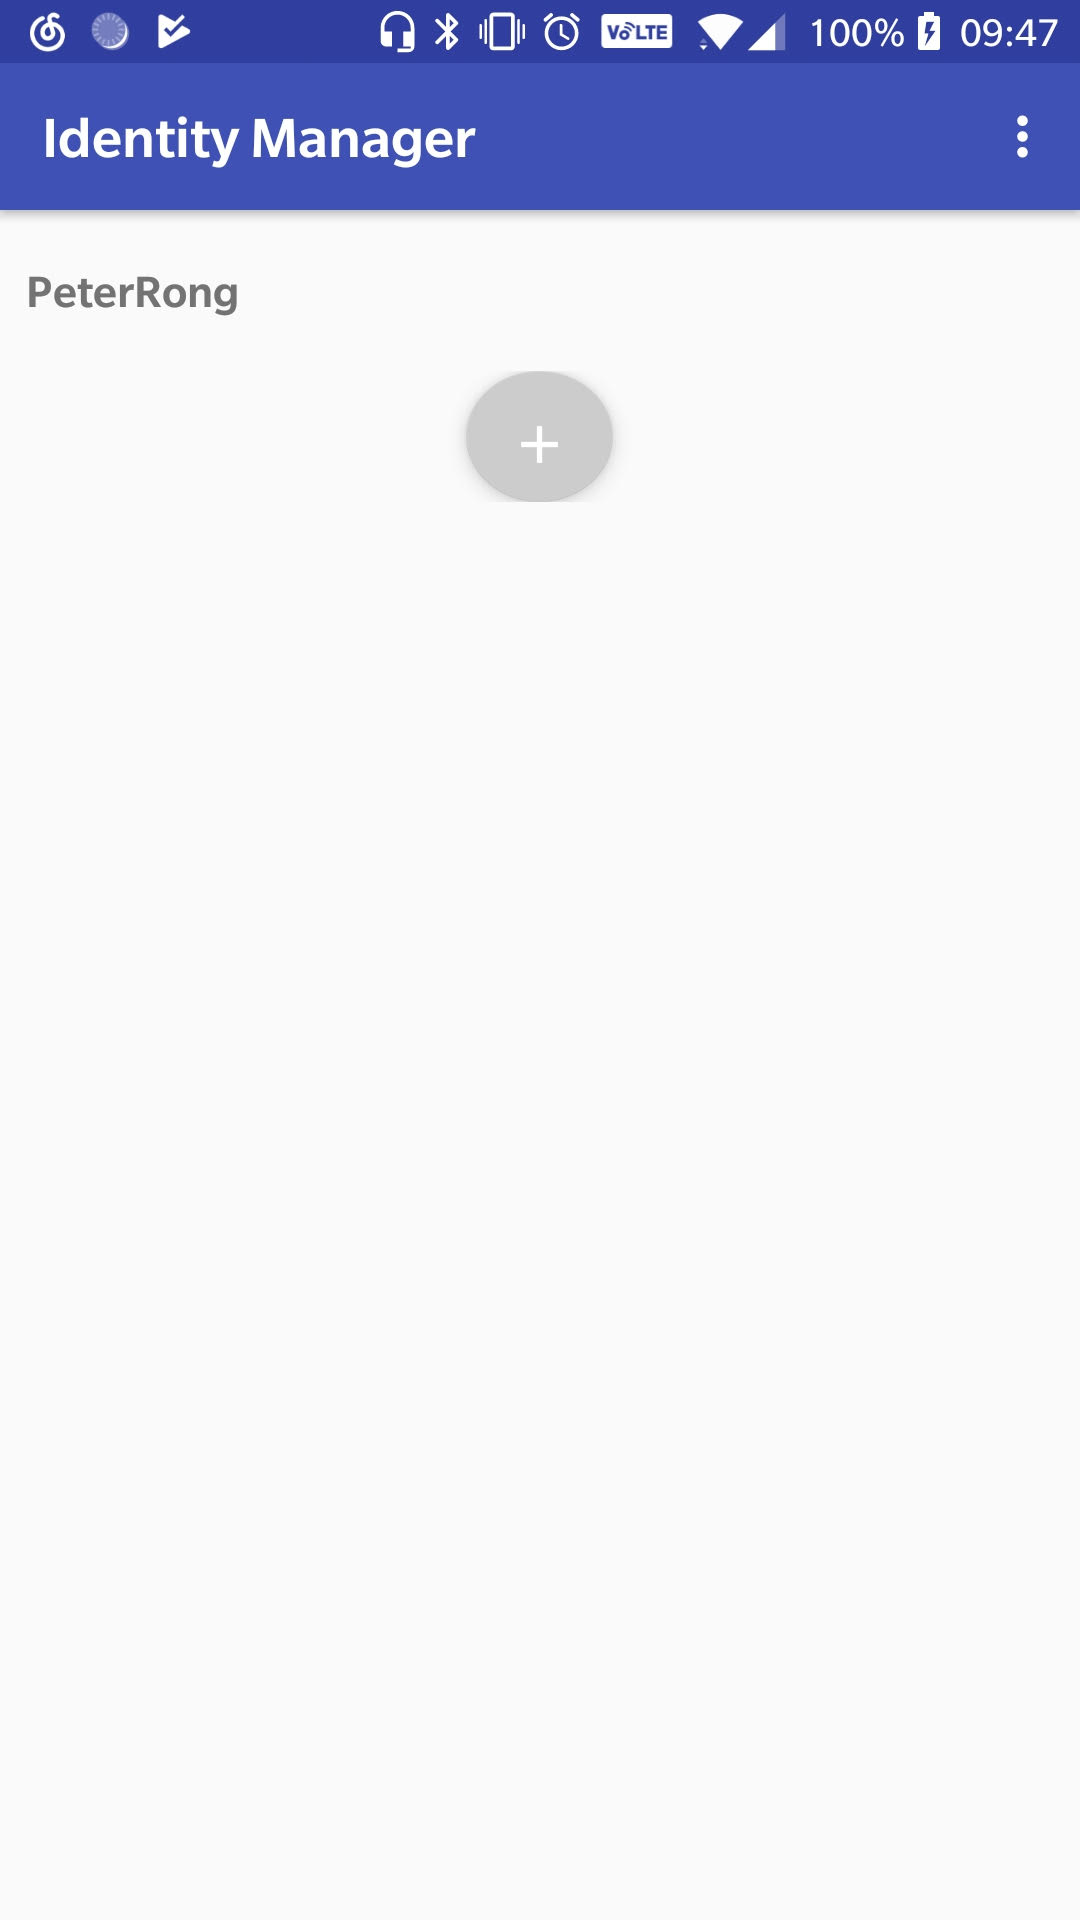
\includegraphics[width=0.24\linewidth]{figures/main-activity.jpg}
	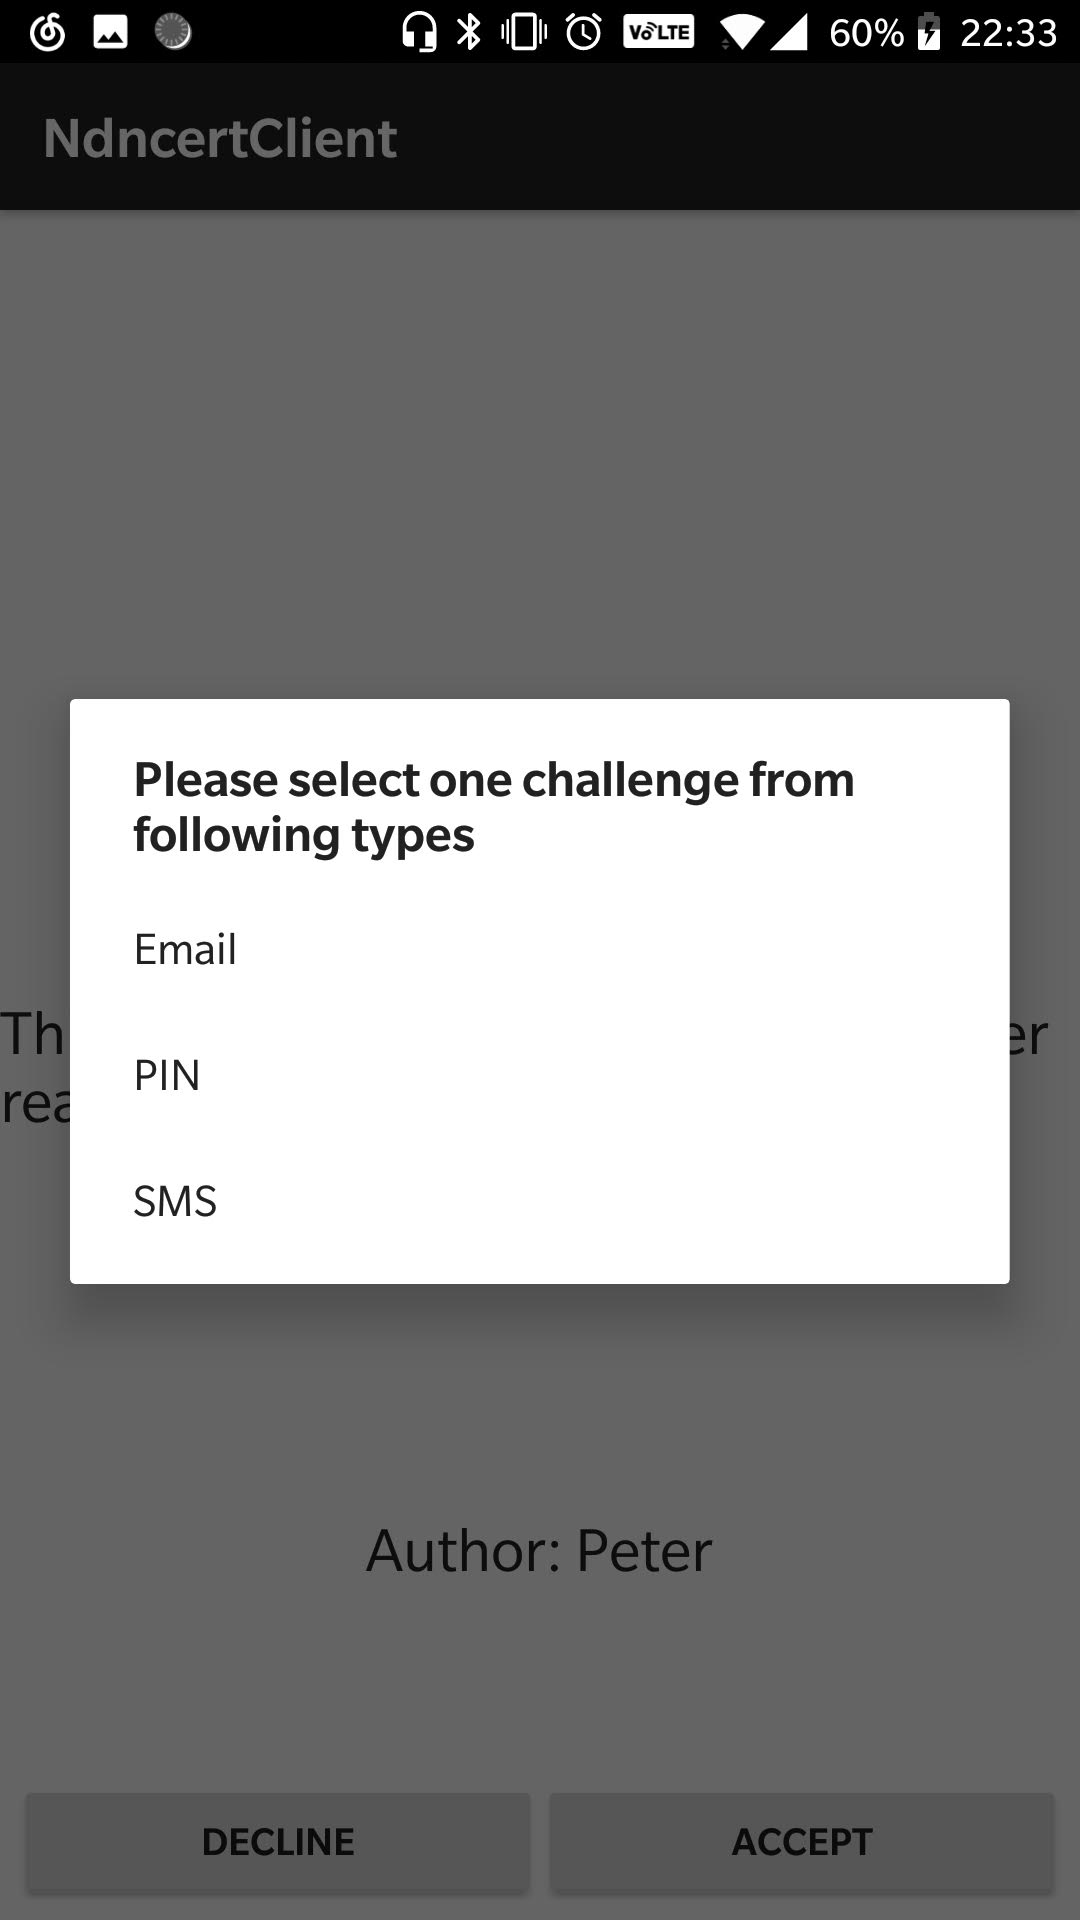
\includegraphics[width=0.24\linewidth]{figures/select.jpg}
	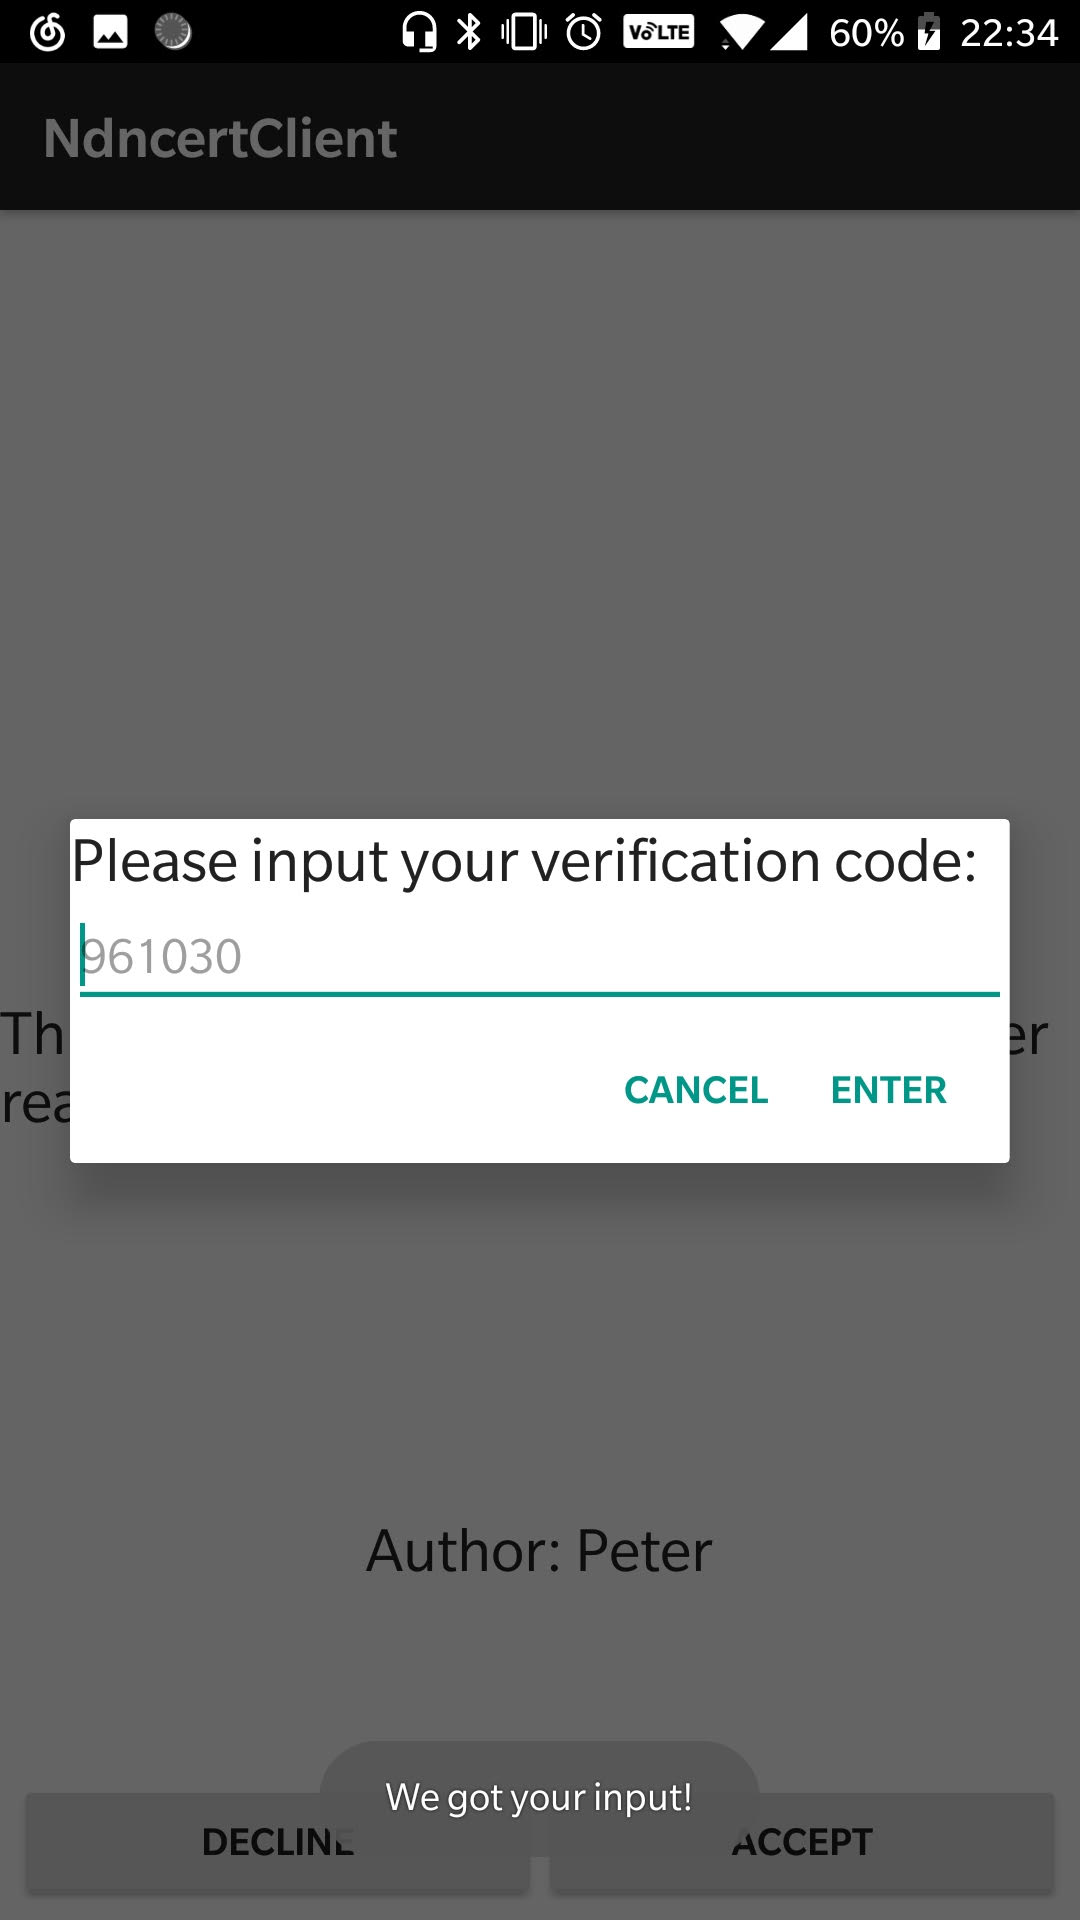
\includegraphics[width=0.24\linewidth]{figures/validate.jpg}
	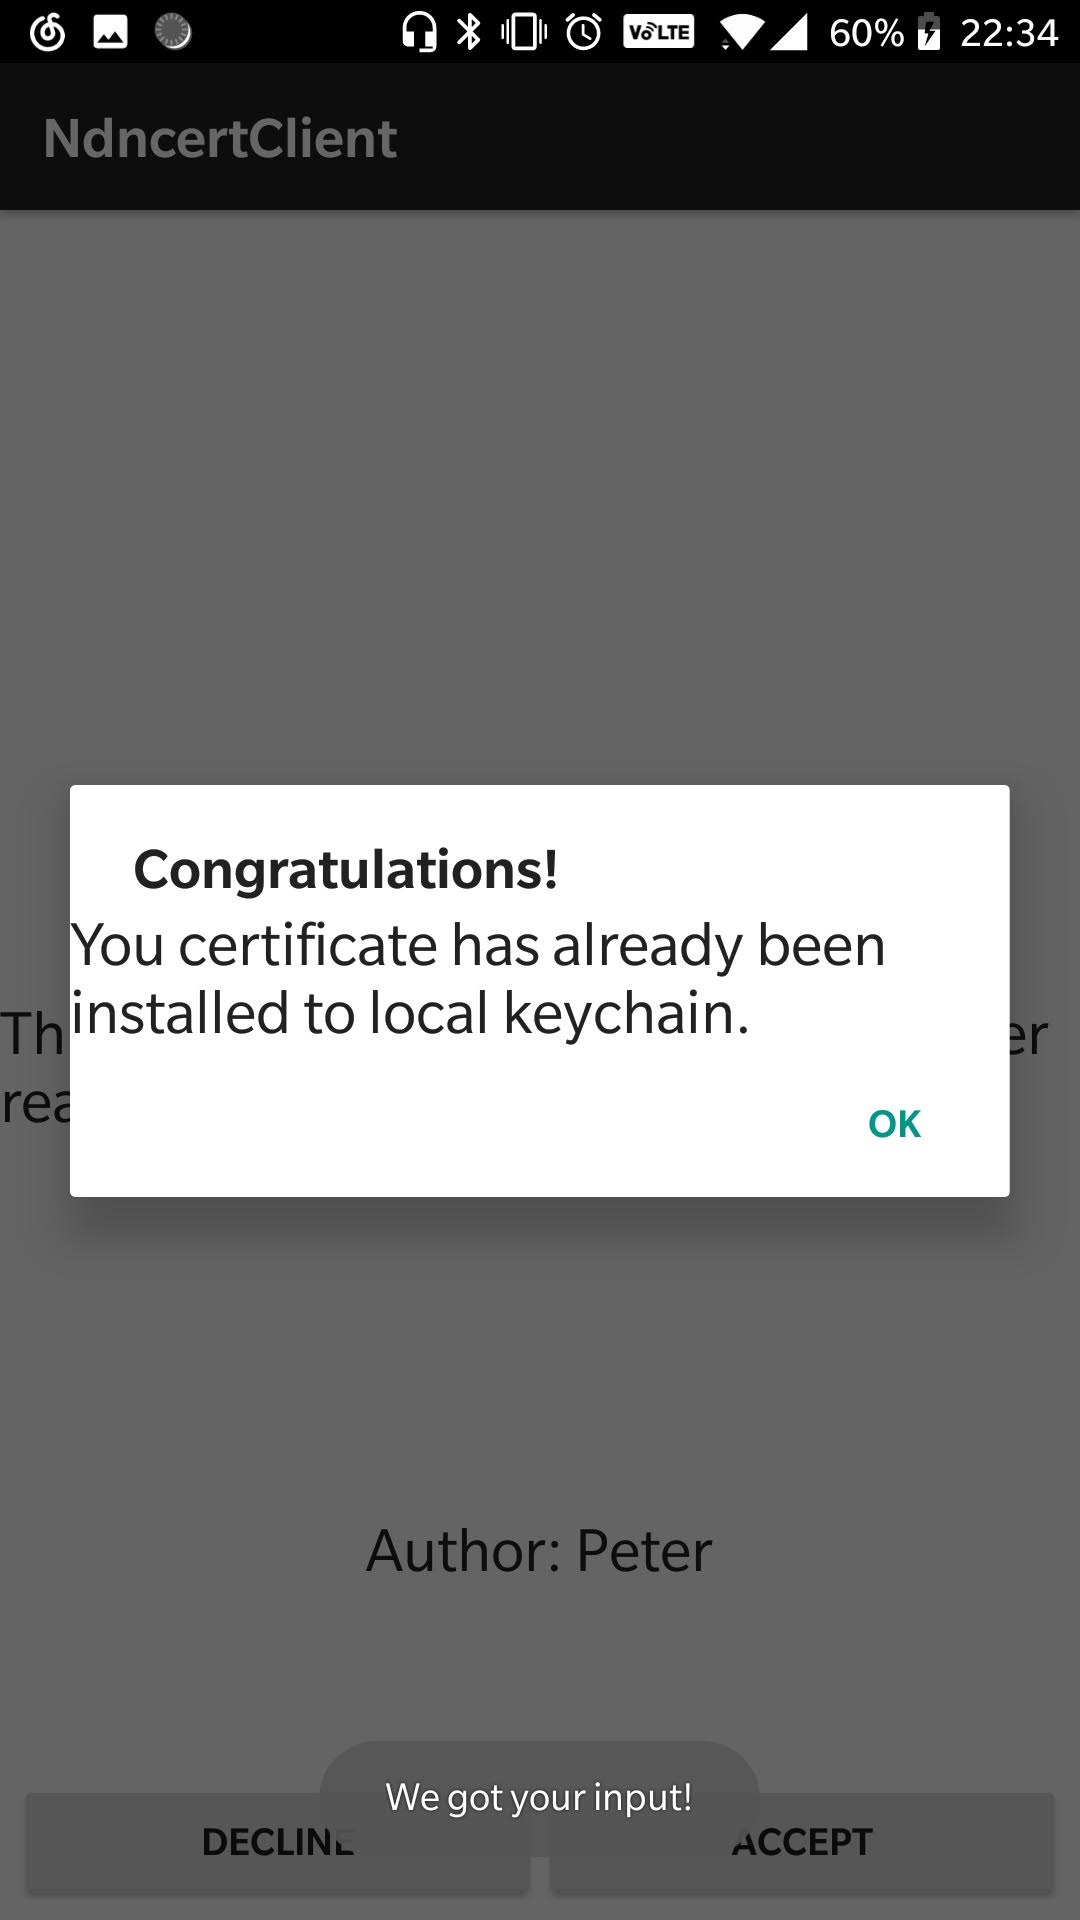
\includegraphics[width=0.24\linewidth]{figures/download.jpg}
\end{minipage}

%----------------------------------------------------------------------------------------
%	CONCLUSIONS
%----------------------------------------------------------------------------------------

%\color{SaddleBrown} % SaddleBrown color for the conclusions to make them stand out

%\section*{Conclusions}

%\color{DarkSlateGray} % Set the color back to DarkSlateGray for the rest of the content

%----------------------------------------------------------------------------------------
%	FORTHCOMING RESEARCH
%----------------------------------------------------------------------------------------

\section*{Future Work}

\par 
	Identity manager is about to be functional, and there are more details that can be added, including:
	\begin{itemize}
		\item identity deleting, 
		\item collision handling when identities have same name,
		\item certificate distribute when requested by other app.
	\end{itemize} 
	There are still coding to do before this app can be used by users.

%----------------------------------------------------------------------------------------
%	REFERENCES
%----------------------------------------------------------------------------------------

\nocite{*} % Print all references regardless of whether they were cited in the poster or not
\bibliographystyle{plain} % Plain referencing style
\bibliography{reference} % Use the example bibliography file sample.bib

%----------------------------------------------------------------------------------------
%	ACKNOWLEDGEMENTS
%----------------------------------------------------------------------------------------

\section*{Acknowledgments}

We would like to thank Lixia Zhang, Arthi Padmanabhan for their help and guidance. Zhiyi Zhang and Alex Afanasyev provided a lot of help when we were developing Android application. Finally, we would like to thanks Ren Sun and CSST for providing such great opportunity.
%----------------------------------------------------------------------------------------

\end{multicols}
\end{document}